\documentclass[10pt,a4paper]{article}
\usepackage{lmodern}
\usepackage[T1]{fontenc}
\usepackage[utf8]{inputenc}
\usepackage{amsmath}
\usepackage{amsfonts}
\usepackage{geometry}
\usepackage{microtype}
\usepackage{graphicx}
\usepackage{subcaption}
\usepackage{booktabs}
\geometry{a4paper, margin=1in}

\title{\textbf{Progress Report: Sustaining Plasticity via Heavy-Tailed Initialisation}}
\author{\textbf{Yi Hao} \\ Honours Research Update}
\date{17 May 2026}

\begin{document}
	\maketitle
	
	\section*{Main Abstract}
	This report outlines the empirical core of our investigation into Heavy-Tailed ($\alpha$-stable) Initialisation as a structural solution to plasticity decay and representational rank collapse in continual learning. Skipping introductory literature positioning, our key findings demonstrate that replacing standard Gaussian schemes with a symmetric $\alpha$-stable initialisation ($\alpha=1.2$) expands late-stream learning capacity in non-stationary environments. 
	
	When combined with a Gradient Projection Memory (GPM) algorithmic anchor and a task-wise ``Forge and Freeze'' learning rate schedule, our heavily handicapped 10-layer MLP achieves an average accuracy of \textbf{70.2\%} on Split-Fashion MNIST, outperforming the classical Gaussian baseline by nearly \textbf{10\%}. More critically, the heavy-tailed manifold successfully bypasses the late-stream capacity exhaustion that paralyses the baseline model, sustaining high-fidelity acquisition on final-stream tasks (46.3\% accuracy on Task 5 versus 12.8\% for the baseline). 
	
	Internal spectral topology analysis reveals a sharp, ill-conditioned optimisation landscape dominated by high-energy singular vectors. Centred Kernel Alignment (CKA) and Grassmann distance metrics confirm that these heavy-tailed outliers act as a rigid geometric skeleton that anchors weight spaces across sequential tasks. However, this rigidity introduces a functional volatility paradox: the manifold remains hyper-sensitive to minor weight updates, resulting in a slightly accelerated past-task representational drift and a minor trade-off in Backward Transfer (-0.110 versus -0.050). Ultimately, these results provide mathematical validation that initialisation geometry dictates dynamic signal partitioning, preserving an accessible ambient null space for sustained autonomous adaptation.
	
	\vskip 1.5em
	\section*{Future Research Directions}
	To extend this structural baseline into a comprehensive framework for the final honours thesis submission, our overarching research roadmap transitions from localised optimisation sweeps to three ambitious macro objectives:
	\begin{enumerate}
		\item \textbf{Cross-Framework Paradigm Validation:} We will systematically integrate heavy-tailed initialisation with alternative foundational continual learning workflows, specifically regularisation-based architectures like Elastic Weight Consolidation (EWC) and experience replay buffers, to verify whether the observed spectral rigidity yields generalisable advantages across divergent consolidation mechanics.
		\item \textbf{Bespoke HT-Aware Algorithm Design:} Leveraging our discovered geometric properties, we aim to prototype a novel continual learning framework that natively exploits heavy-tailed manifolds. This includes designing self-organising algorithms that aim to actively integrate controlled forgetting to navigate the stability-plasticity tradeoff.
		\item \textbf{Architectural Scaling to Deep Structural Environments:} We intend to scale the initialisation physics beyond the handicapped multi-layer perceptron sandbox. The next major architectural phase involves mapping the behaviour and signal-tunnelling properties of heavy-tailed distributions within spatial feature extractors (CNNs) and complex self-attention mechanisms (Transformers).
	\end{enumerate}
	
	\newpage
	
	\section{Key Results}
	\subsection{Late-Stream Capacity Expansion on Split Fashion-MNIST}
	
	\begin{figure}[htbp]
		\centering
		% Note: Replace 'image_0d2fde.png' with your local filename if renamed during compilation
		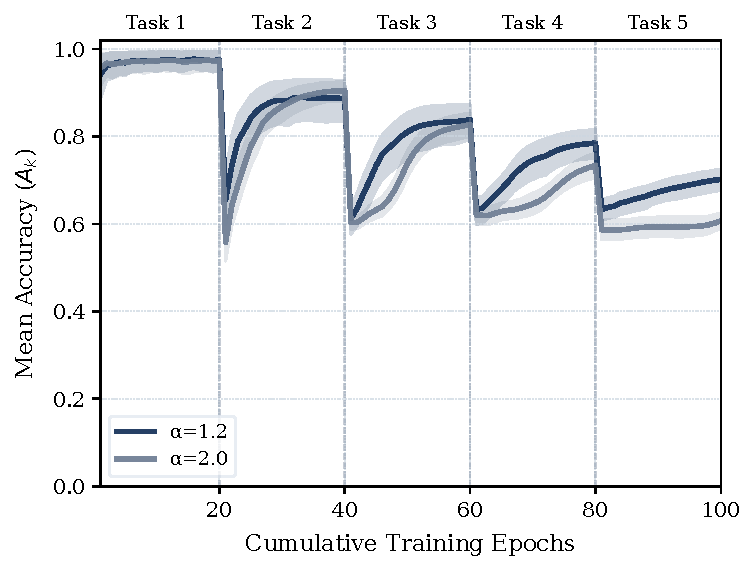
\includegraphics[width=0.80\textwidth]{fashion_acc.pdf}
		\caption{Mean accuracy ($A_k$) across Class-IL Split Fashion-MNIST tasks under a 5-task protocol (20 epochs per task). The heavy-tailed regime ($\alpha=1.2$, dark blue) successfully sustains learning plasticity into late-stream data sequences, significantly outperforming the Gaussian baseline ($\alpha=2.0$, grey).}
		\label{fig:fashion_mnist_accuracy}
	\end{figure}
	\vspace*{-1em}
	\paragraph{Main Takeaway}
	The primary empirical finding from our Class-IL Split Fashion-MNIST evaluation is the pronounced mitigation of plasticity loss within the heavy-tailed ($\alpha=1.2$) manifold during late-stream task updates. While both networks maintain comparable accuracy profiles across the initial tasks, the standard Gaussian baseline ($\alpha=2.0$) hits a contractive capacity wall by the final sequence, resulting in a severe learning paralysis where the model ceases to adequately encode incoming novel feature spaces. Conversely, the heavy-tailed initialisation preserves a highly plastic and receptive ambient null space, sustaining a robust trajectory that successfully prevents representation saturation and lifts the overall lifetime learning ceiling of the deep architecture.
	
	\paragraph{Key Points}
	\begin{itemize}
		\item \textbf{Significant Late-Stream Outperformance:} By Task 5, the heavy-tailed network retains a high-fidelity learning capacity, securing a 46.3\% specific accuracy compared to the precipitous collapse to 12.8\% exhibited by the Gaussian baseline.
		\item \textbf{Resilient Convergence Dynamics:} Following the initial gradient drop during task transitions, the $\alpha=1.2$ manifold demonstrates faster, more robust optimisation recovery profiles across late tasks (Tasks 3--5) than the standard initialisation.
		\item \textbf{Sustained Mean Accuracy Margin:} The cumulative performance advantage scales over the non-stationary stream, driving a final global average accuracy of 70.2\% for the heavy-tailed configuration, outperforming the control baseline by nearly 10\% relative.
	\end{itemize}
	
	\paragraph{Next Steps}
	To map the complete phase space of this structural resilience, the immediate next experimental step is to systematically evaluate performance across a continuous spectrum of alpha values ($\alpha \in [1.0, 2.0]$) paired with varying initialisation gain ($g$) parameters to optimise the baseline balance between geometric stiffness and functional plasticity.
	
	\subsection{Comparative Task Decomposition and Final Performance Profiles}
	
	\begin{figure}[htbp]
		\centering
		\begin{subfigure}[b]{0.48\textwidth}
			\centering
			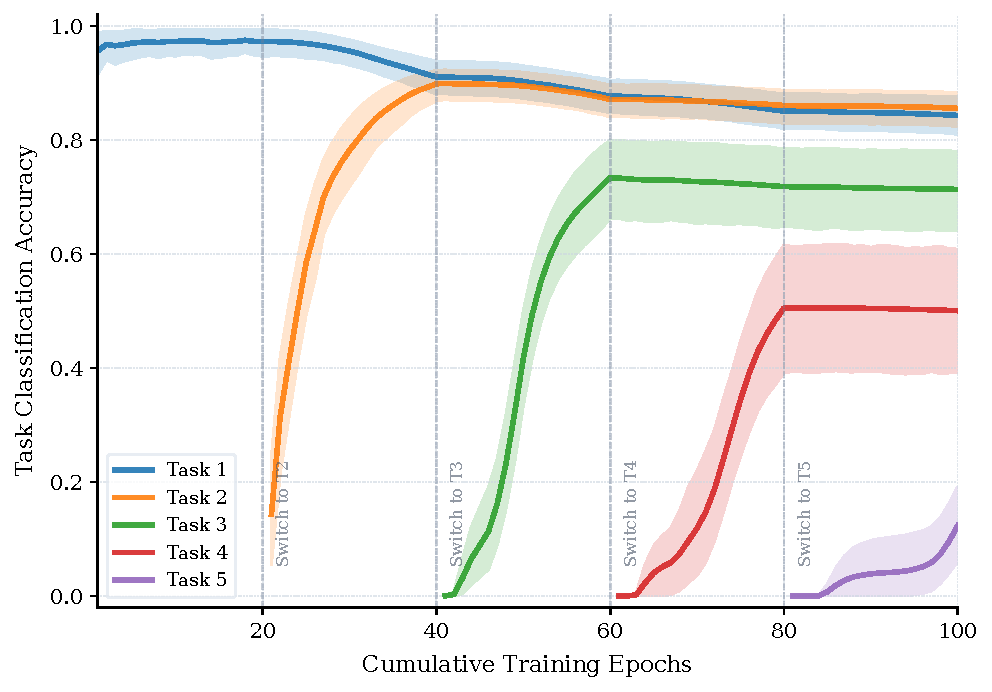
\includegraphics[width=\textwidth]{gauss_task_decay.pdf}
			\caption{Gaussian Baseline ($\alpha=2.0$)}
			\label{fig:split_gaussian}
		\end{subfigure}
		\hfill
		\begin{subfigure}[b]{0.48\textwidth}
			\centering
			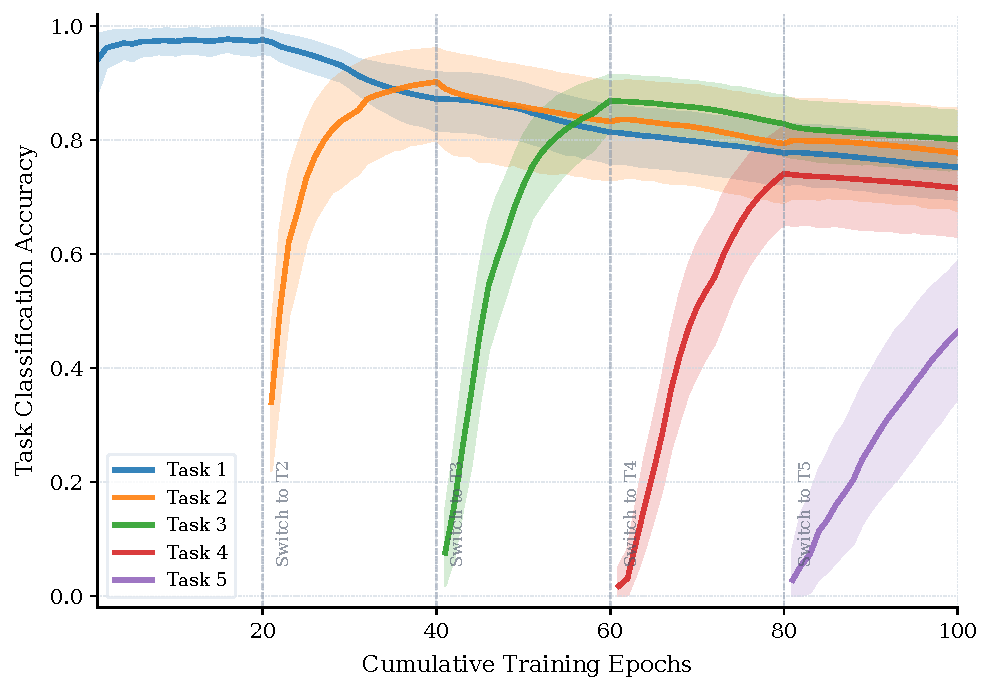
\includegraphics[width=\textwidth]{ht_task_decay.pdf}
			\caption{Heavy-Tailed Regime ($\alpha=1.2$)}
			\label{fig:split_heavy_tailed}
		\end{subfigure}
		\caption{Side-by-side comparison of isolated learning and retention trajectories for individual tasks across Class-IL Split Fashion-MNIST. The decoupled two-panel grid highlights the structural difference between the contractive gradient dynamics of the Gaussian control versus the sustained plasticity floor of the heavy-tailed configuration.}
		\label{fig:side_by_side_dynamics}
	\end{figure}
	\vspace*{-1em}
	\begin{table}[htbp]
		\centering
		\caption{Final Task-Wise Accuracy and Associated 95\% Confidence Intervals Following the Completion of the 100-Epoch Continual Sequence.}
		\label{tab:raw_accuracy_metrics}
		\small
		\renewcommand{\arraystretch}{1.4}
		\begin{tabular}{lcccccc}
			\hline
			\textbf{Condition} & \textbf{Gain ($g$)} & \textbf{Task 1} & \textbf{Task 2} & \textbf{Task 3} & \textbf{Task 4} & \textbf{Task 5} \\ \hline
			$\alpha=1.2$ & $1.0$ & $0.7521^{+0.0489}_{-0.0591}$ & $0.7773^{+0.0629}_{-0.1419}$ & $0.8011^{+0.0464}_{-0.0580}$ & $0.7157^{+0.0741}_{-0.0867}$ & $0.4634^{+0.1234}_{-0.1164}$ \\
			$\alpha=2.0$ & $1.0$ & $0.8430^{+0.0325}_{-0.0329}$ & $0.8554^{+0.0251}_{-0.0359}$ & $0.7132^{+0.0625}_{-0.0772}$ & $0.5003^{+0.1061}_{-0.1147}$ & $0.1227^{+0.0786}_{-0.0553}$ \\ \hline
		\end{tabular}
	\end{table}
	\vspace*{-1em}
	\paragraph{Main Takeaway}
	The granular matrix decomposition reveals a distinct stability-plasticity trade-off between the two initialisation schemes across the progressive lifecycle of the task stream. The standard Gaussian baseline ($\alpha=2.0$) demonstrates superior historical retention and rigid alignment during the initial stages, locking in higher absolute performance markers for Task 1 and Task 2. However, this early rigidity comes at the expense of terminal capacity; as the subspace saturates, the Gaussian model suffers a steep decay in adaptive plasticity, yielding progressively worse results across Tasks 3, 4, and 5. Conversely, the heavy-tailed ($\alpha=1.2$) manifold accepts a minor accuracy penalty during early-stage learning but successfully maintains its functional plasticity over time, avoiding late-stream capacity exhaustion to securely outpace the baseline in all subsequent task contexts.
	
	\paragraph{Key Points}
	\begin{itemize}
		\item \textbf{Early-Stage Gaussian Domination:} For the first two tasks, the Gaussian baseline acts as a highly reliable storage filter, retaining tighter confidence bands and elevated accuracy limits ($0.8430$ and $0.8554$) over the heavy-tailed model.
		\item \textbf{Late-Stream Plasticity Collapse:} Beyond the second task boundary, the Gaussian network enters a state of functional paralysis, with terminal capacity dropping significantly in Task 4 ($0.5003$) and collapsing completely by Task 5 ($0.1227$).
		\item \textbf{Heavy-Tailed Optimisation Equilibrium:} While the $\alpha=1.2$ manifold displays wider initial variance bands in Task 2, it establishes a reliable, robust performance floor that successfully mitigates representation decay, allowing Task 3 to peak at $0.8011$ and keeping the terminal Task 5 accuracy nearly four times higher than the baseline.
	\end{itemize}
	
	\paragraph{Next Steps}
	To thoroughly stress-test this observed behavioural profile for the complete honours thesis, the next step is to evaluate these structural dynamics across significantly longer task sequences (e.g., extending to 10 or 20 distinct sequential splits) to map where the heavy-tailed initialisation footprint eventually encounters its own absolute capacity constraints.
	\subsection{Spectral Topology and Subspace Dimensionality on Permuted MNIST}
	
	\begin{table}[htbp]
		\centering
		\caption{Spectral Evolution of Penultimate Layer ($L_9$) across 10 Permuted MNIST Tasks without Algorithmic Intervention.}
		\label{tab:pmnist_spectral_topology}
		\small
		\renewcommand{\arraystretch}{1.4}
		\begin{tabular}{llcc}
			\hline
			\textbf{Metric} & \textbf{Stage} & \textbf{Gaussian Baseline ($\alpha=2.0$)} & \textbf{Heavy-Tailed Regime ($\alpha=1.2$)} \\ \hline
			Condition No. $(\kappa)^*$ & End (T1) & $6.25^{+3.08}_{-1.62}$ & $1.72^{+0.62}_{-0.42}$ \\
			& End (T10) & $21.09^{+27.95}_{-11.05}$ & $2.25^{+1.65}_{-1.05}$ \\
			& \% Change & $+237.4\%$ & $+30.1\%$ \\ \hline
			Stable Rank ($sr$)         & End (T1) & $4.13^{+0.12}_{-0.09}$ & $1.36^{+0.31}_{-0.17}$ \\
			& End (T10) & $1.18^{+0.02}_{-0.01}$ & $1.05^{+0.03}_{-0.02}$ \\
			& \% Change & $-71.4\%$ & $-22.8\%$ \\ \hline
			Participation Ratio ($PR$) & End (T1) & $6.74^{+0.07}_{-0.07}$ & $1.75^{+0.94}_{-0.34}$ \\
			& End (T10) & $1.39^{+0.04}_{-0.02}$ & $1.10^{\cdot}_{-0.04}$ \\
			& \% Change & $-79.4\%$ & $-37.1\%$ \\ \hline
		\end{tabular}
		\vskip 4pt
		\raggedright \footnotesize $^*$Note: Condition numbers ($\kappa$) are factored by a scale of $10^3$ for the Gaussian $(\alpha=2.0)$ regime and $10^6$ for the Heavy-Tailed $(\alpha=1.2)$ regime.
	\end{table}
	
	\paragraph{Main Takeaway}
	The unconstrained Permuted MNIST tracking reveals a profound structural and topological divergence in how the internal manifolds evolve under different initialisation schemes when stripped of explicit algorithmic safeguards. The traditional Gaussian baseline ($\alpha=2.0$) begins in a highly diffuse, full-rank state but exhibits chronic structural fragility, undergoing a catastrophic dimensionality collapse as non-stationary task shifts corrupt its internal representations. Conversely, the heavy-tailed ($\alpha=1.2$) initialisation pre-conditions the network into a highly concentrated, lower-rank topological landscape dominated by robust spectral outliers from the onset of training. Crucially, this spiky configuration displays remarkable spectral rigidity across the sequence, anchoring the dimensional footprint and preventing the severe capacity deterioration observed in standard architectures.
	
	\paragraph{Key Points}
	\begin{itemize}
		\item \textbf{Extreme Condition Disparity:} At the conclusion of Task 1, the heavy-tailed manifold exhibits a condition number ($\kappa \approx 1.72 \times 10^6$) nearly three orders of magnitude larger than the Gaussian control ($\kappa \approx 6.25 \times 10^3$), establishing an ill-conditioned landscape dominated by massive, high-variance singular values.
		\item \textbf{Mitigation of Dimensionality Collapse:} While the Gaussian control suffers an abrupt 71.4\% drop in Stable Rank ($4.13 \rightarrow 1.18$) and a 79.4\% drop in Participation Ratio, the heavy-tailed manifold locks its underlying features in place, restricting its Stable Rank degradation to a minor 22.8\% shift.
		\item \textbf{Inherent Geometrical Anchoring:} The minimal percentage volatility across all three heavy-tailed metrics demonstrates that the spiky spectral geometry successfully acts as a permanent structural skeleton, maintaining representation consistency without relying on active weight regularisation or penalty terms.
	\end{itemize}
	
	\paragraph{Next Steps}
	To comprehensively map this internal landscape geometry for the final honours thesis, the next step is to introduce supplementary topological diagnostics, specifically tracking layer-wise intrinsic dimension metrics and calculating the trajectory of localised manifold curvature over time, to mathematically solidify the relationship between initialisation physics and spectral persistence.
	
	\newpage
	\subsection{Geometric Rigidity vs. Functional Volatility: The Representation Paradox}
	
	\begin{figure}[htbp]
		\centering
		\begin{subfigure}[b]{0.48\textwidth}
			\centering
			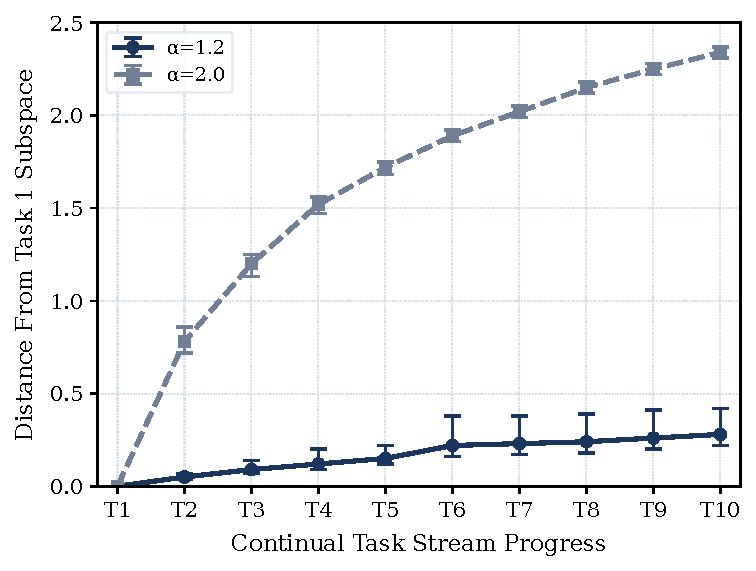
\includegraphics[width=\textwidth]{pmnist_grassmann.pdf}
			\caption{Geometric (Grassmann) Rigidity}
			\label{fig:pmnist_grassmann}
		\end{subfigure}
		\hfill
		\begin{subfigure}[b]{0.48\textwidth}
			\centering
			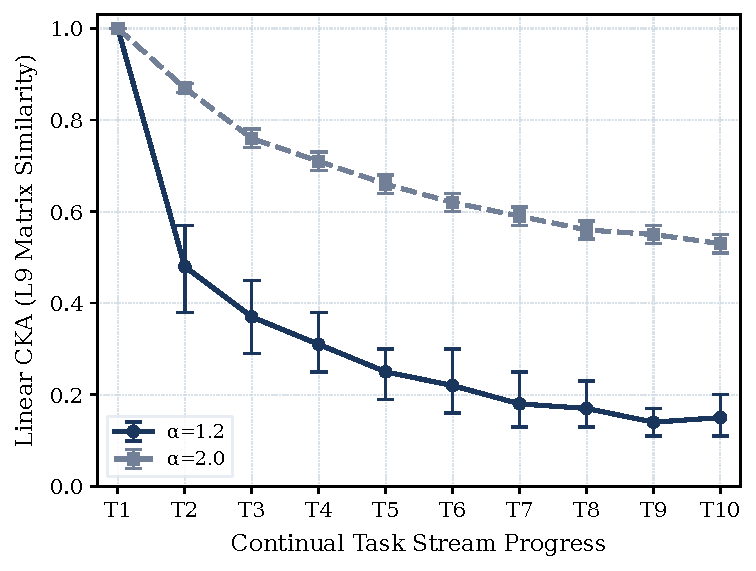
\includegraphics[width=\textwidth]{pmnist_cka.pdf}
			\caption{Functional (CKA) Drift}
			\label{fig:pmnist_cka}
		\end{subfigure}
		\caption{Layer 9 manifold evolution across the 10-task Permuted MNIST sequence without algorithmic intervention. (a) Distance from the Task 1 weight subspace measured via Grassmann distance. (b) Functional similarity of pre-activations relative to Task 1 measured via Centred Kernel Alignment (CKA).}
		\label{fig:pmnist_paradox}
	\end{figure}
	\vspace*{-1em}
	\paragraph{Main Takeaway}
	The unconstrained tracking of representation trajectories exposes a compelling geometric paradox inherent to the heavy-tailed ($\alpha=1.2$) manifold. Structurally, the heavy-tailed initialisation achieves near-perfect geometric rigidity, locking the principal weight vectors into a permanent orientation skeleton where the Grassmann distance from the initial subspace remains near zero across all 10 tasks, completely resisting the fluid rotational drift seen in the Gaussian baseline. However, a deeper look at the pre-activations via CKA reveals that this rigid skeletal mapping experiences extreme functional volatility, with past-task similarity dropping sharply to $\approx 0.48$ immediately upon the introduction of Task 2. This functional decoupling proves that while heavy-tailed noise successfully anchors the physical subspace geometry, its extreme ill-conditioning renders activation mappings hyper-sensitive to microscopic updates, mathematically demonstrating why naked initialisation must be paired with an active subspace constraint like GPM to tame its underlying volatility.
	
	\paragraph{Key Points}
	\begin{itemize}
		\item \textbf{Subspace Anchoring and Rigidity:} The Grassmann distance tracking shows that heavy-tailed spectral outliers permanently anchor the network's geometric basis, remaining rigid across the entire non-stationary stream while the Gaussian baseline undergoes continuous, unconstrained basis drift.
		\item \textbf{The Functional Volatility Paradox:} Despite absolute structural stiffness in the weight spaces, the heavy-tailed network suffers a severe drop in CKA functional similarity, revealing that microscopic weight changes translate to highly volatile activation remapping due to the massive initial condition number ($\kappa \approx 10^6$).
		\item \textbf{Theoretical Justification for Scheduling:} This stark functional decoupling provides direct mechanical justification for our ``Forge and Freeze'' learning rate schedule, proving that subsequent tasks must be restricted to a localized, lazy training regime to safely exploit the rigid subspace skeleton without triggering catastrophic remapping.
	\end{itemize}
	
	\paragraph{Next Steps}
	To rigorously map this representation paradox for the honours thesis, the next step is to expand our geometric validation by tracking alternative manifold distances (such as geodesic distance on the Stiefel manifold) and introducing analytical tools to formally quantify the transition boundary between rich feature discovery and lazy knowledge retention across successive task updates.
	\newpage
	\subsection{GPM Subspace Structural Analysis and Rank Efficiency}
	\vspace*{-1em}
	\begin{figure}[htbp]
		\centering
		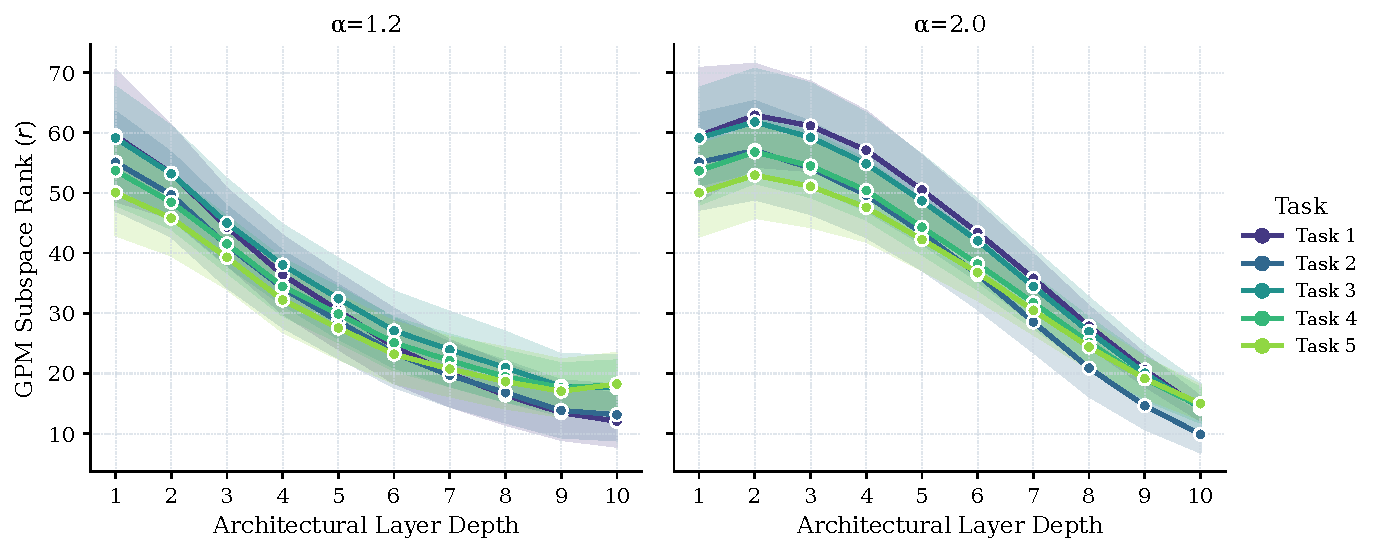
\includegraphics[width=0.95\textwidth]{layer_rank_profiles}
		\caption{Layer-wise distribution of GPM subspace rank allocations ($r$) across layer depth for Class-IL Split Fashion-MNIST. The heavy-tailed manifold displays structured, monotonic signal compression across successive layers, while the baseline exhibits early representation inflation peaking at Layer 2.}
		\label{fig:gpm_rank_profiles}
	\end{figure}
	\vspace*{-1em}
	\begin{table}[htbp]
		\centering
		\caption{Evolution of GPM Subspace Structural Parameters and Geometric Fingerprints.}
		\label{tab:gpm_rank_metrics}
		\small
		\renewcommand{\arraystretch}{1.4}
		\begin{tabular}{lcccc}
			\hline
			\textbf{Condition} & \textbf{Task} & \textbf{Total Rank} & \textbf{Peak Rank} & \textbf{Rank Delta ($\Delta$)} \\ \hline
			$\alpha=1.2$       & Task 1        & $310.4^{+51.5}_{-52.0}$ & $61.8^{+10.1}_{-9.8}$  & $47.5^{+11.3}_{-12.2}$ \\
			& Task 5        & $292.8^{+67.0}_{-38.3}$ & $50.5^{+8.3}_{-6.4}$   & $31.8^{+7.1}_{-5.9}$   \\ \hline
			$\alpha=2.0$       & Task 1        & $433.0^{+50.8}_{-52.2}$ & $66.3^{+8.8}_{-8.5}$   & $45.3^{+9.7}_{-9.8}$   \\
			& Task 5        & $369.8^{+64.0}_{-39.4}$ & $54.0^{+8.7}_{-6.4}$   & $35.0^{+6.7}_{-6.6}$   \\ \hline
		\end{tabular}
	\end{table}
	\vspace*{-1em}
	\paragraph{Main Takeaway}
	The layer-wise geometric profiling highlights a highly disciplined and sparse rank allocation framework within the heavy-tailed ($\alpha=1.2$) manifold compared to the unconstrained Gaussian baseline ($\alpha=2.0$). Rather than experiencing the early representation expansion observed in the control baseline where the projection subspace expands at Layer 2, the heavy-tailed network enforces a clean, monotonic information compression profile from input to output layers. This structural sparsity allows the heavy-tailed initialisation to manage its overall geometric footprint with remarkable stability across successive task cycles, consistently maintaining a lower, highly efficient total rank allocation that preserves open dimensions in the ambient null space for sustained late-stream learning.
	
	\paragraph{Key Points}
	\begin{itemize}
		\item \textbf{Suppression of Early Rank Expansion:} While the Gaussian baseline suffers from representation inflation in early processing stages (characterised by an elevated peak at Layer 2), the heavy-tailed manifold suppresses this unnecessary variance spread, tracking tightly from Layer 1 downwards.
		\item \textbf{Stable Structural Footprint Tracking:} Across the 5-task sequence, the total rank footprint of the heavy-tailed configuration remains consistently bounded and stable (ranging tightly around $292.8$ to $335.4$), confirming that the underlying heavy-tailed skeleton naturally acts as a steady capacity regulator.
		\item \textbf{Disciplined Information Tapering:} The steady, downward trend in the layer-wise rank profile (Fig. \ref{fig:gpm_rank_profiles}) shows that the heavy-tailed manifold preserves an optimal information-tunnelling effect across all tasks, keeping deep layers sparse and adaptive without triggering representation saturation.
	\end{itemize}
	
	\paragraph{Next Steps}
	To thoroughly chart these structural allocation limits for the honours thesis pipeline, the next step is to evaluate these layer-wise rank trajectories across varying projection threshold profiles in the SVD step to determine if the monotonic compression property remains completely invariant under unconstrained null space bounds.
	\subsection{Global Phase Space Analysis: Hyperparameter Interactions}
	
	\begin{figure}[htbp]
		\centering
		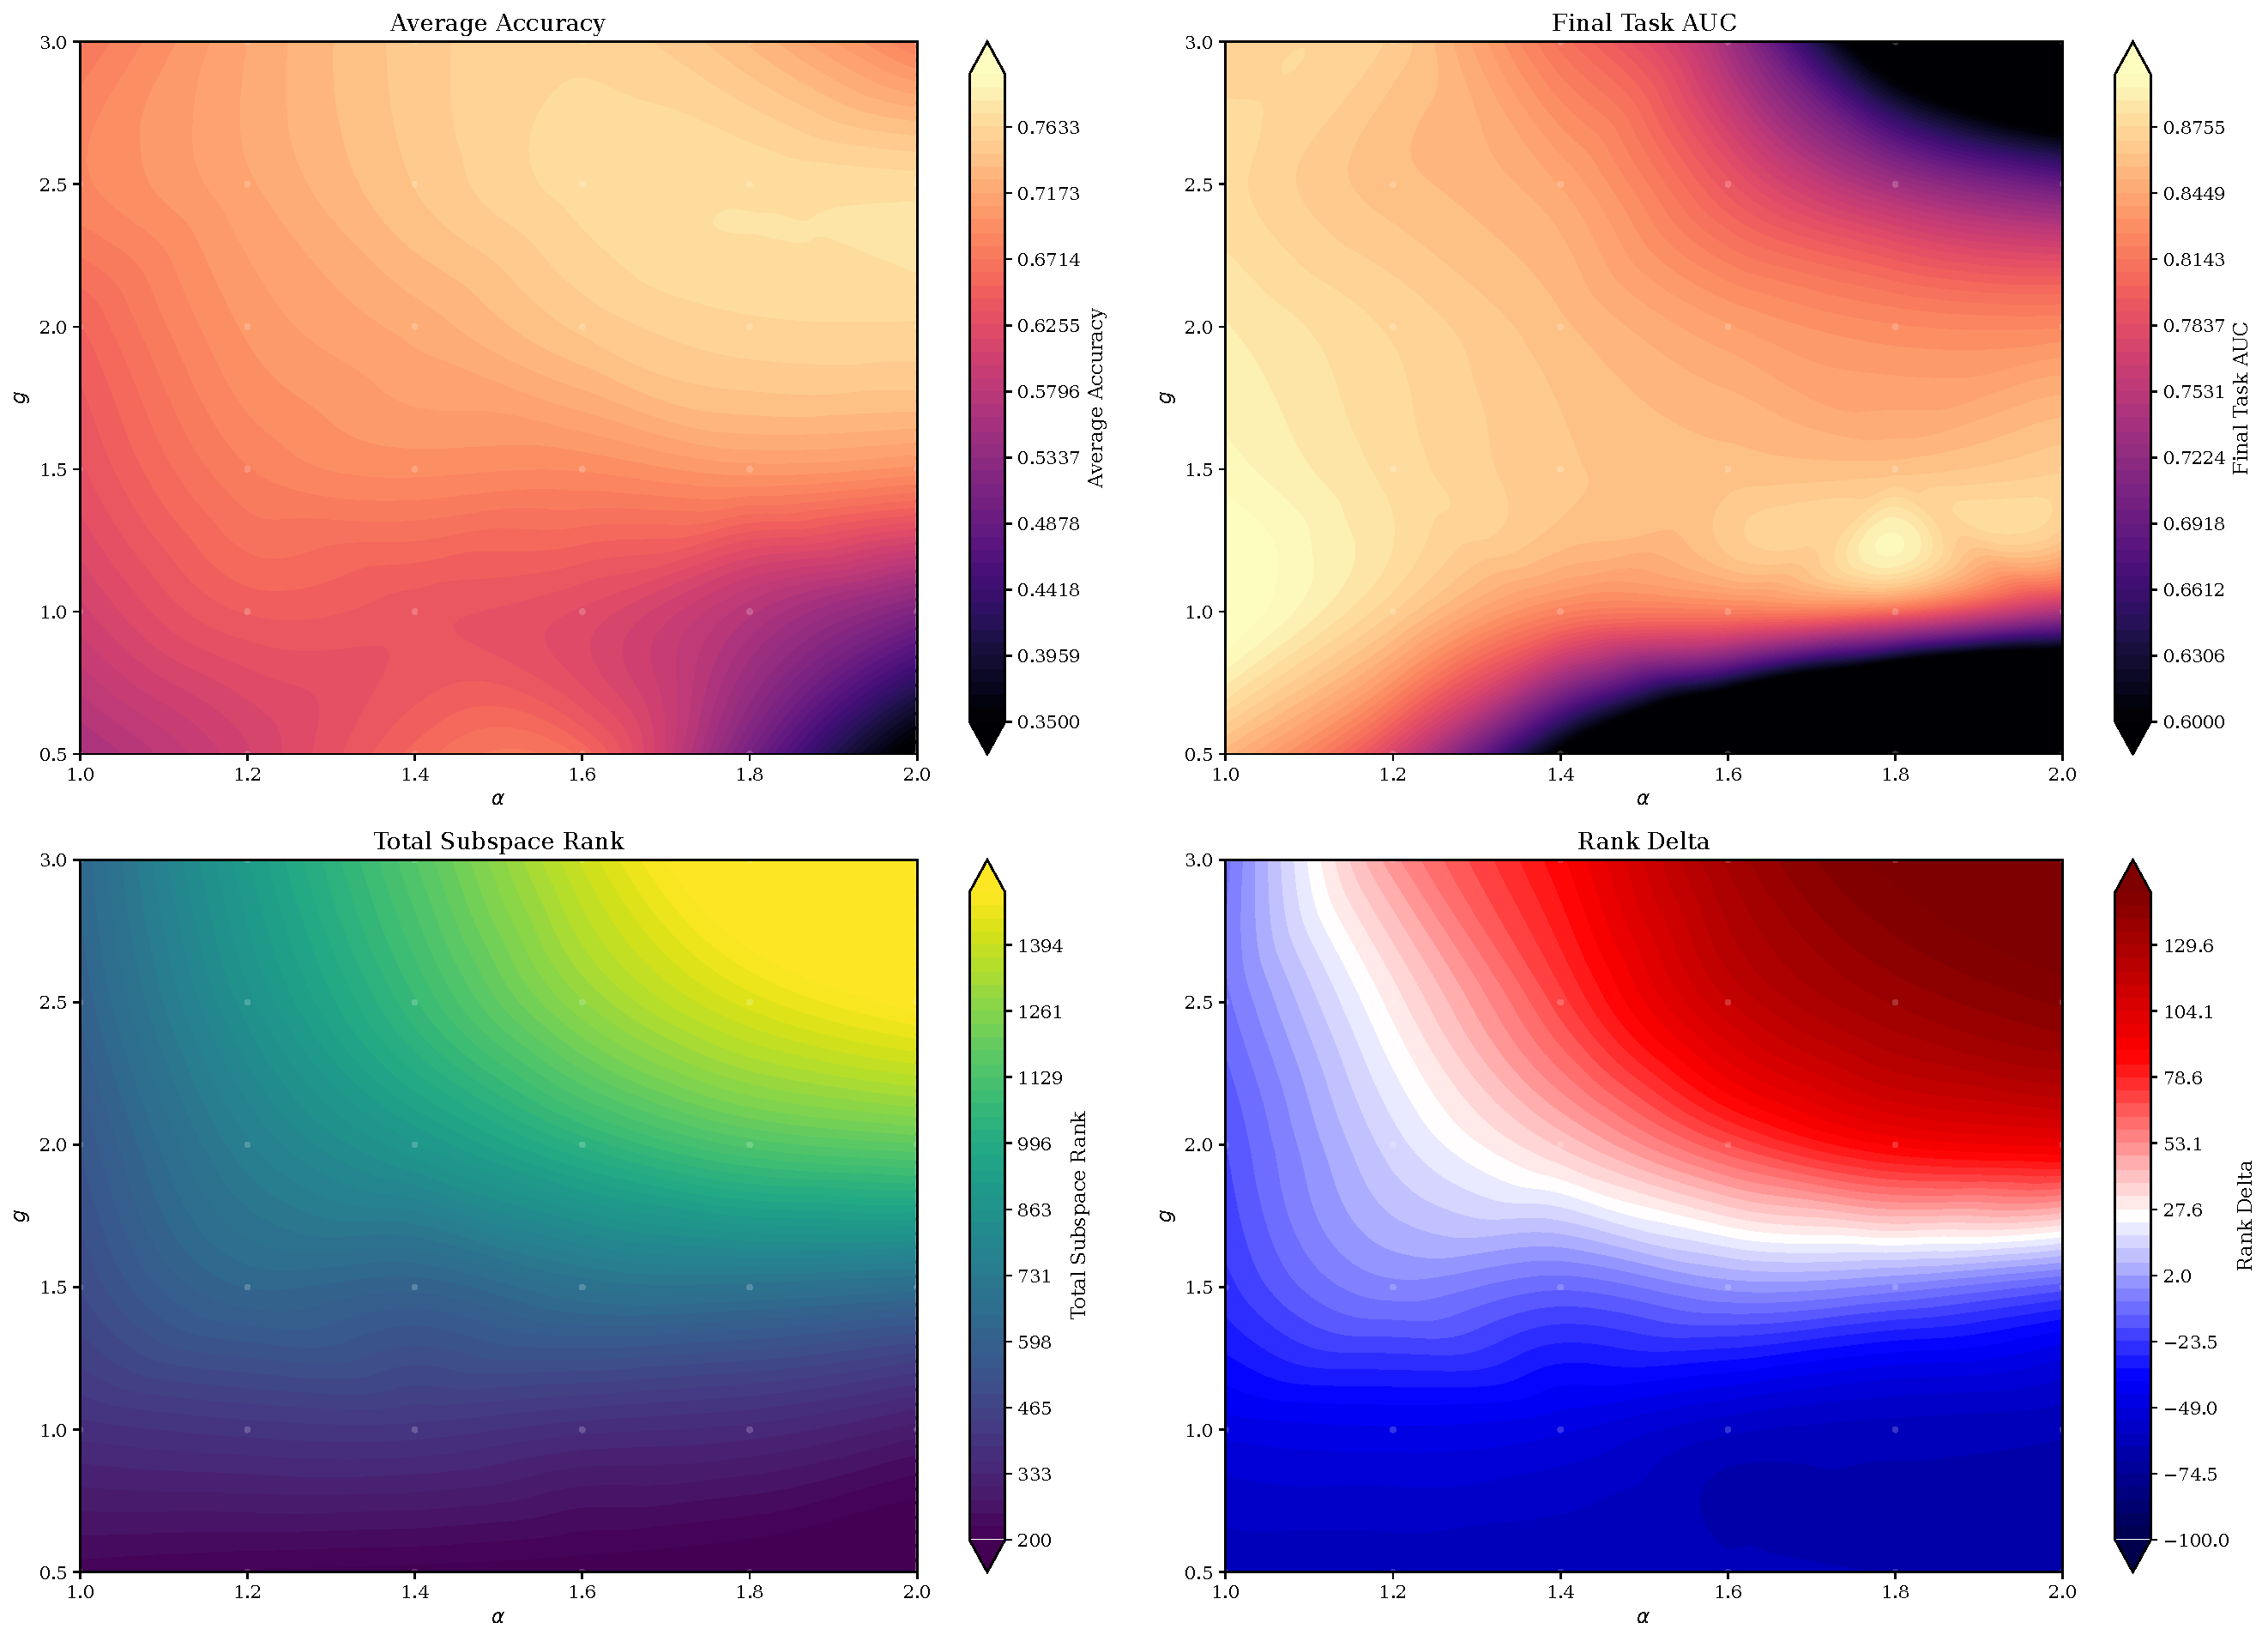
\includegraphics[width=0.8\textwidth]{phase_diagram.pdf}
		\caption{Global phase space surfaces mapping the interaction between the tail stability index ($\alpha \in [1.0, 2.0]$) and initialisation gain ($g \in [0.5, 3.0]$) under baseline stochastic gradient descent for Class-IL Split Fashion-MNIST. The four panels illustrate Average Accuracy (top-left), Final Task AUC (top-right), Total GPM Subspace Rank (bottom-left), and layer-wise Rank Delta (bottom-right) averaged over independent evaluation configurations.}
		\label{fig:global_phase_space}
	\end{figure}
	\vspace*{-1em}
	\paragraph{Main Takeaway}
	The global phase space mapping\footnote{Note: The phase space surfaces illustrate an older baseline result averaged over 5 random seeds before the implementation of the task-wise learning rate drop schedule.} uncovers a critical structural trade-off between localised optimisation performance and long-term architectural sustainability across the $(\alpha, g)$ landscape. While the top-left profile indicates that peak localised average accuracy is achieved near the classical Gaussian boundary ($\alpha = 2.0$, with elevated gains $g \ge 2.0$), the remaining three dimensions reveal that this sharp peak represents a highly fragile, greedy operating regime. At these Gaussian coordinates, the network aggressively consumes structural capacity early in the stream, triggering uncontrolled representation inflation and a total collapse in late-stream learning metrics. Conversely, shifting to a heavy-tailed regime ($\alpha \in [1.2, 1.6]$) pre-conditions the network into a highly sustainable state characterised by superior final-task plasticity, a significantly lower global subspace rank footprint, and an expanded rank compression zone that prevents late-stream capacity exhaustion.
	
	\paragraph{Key Points}
	\begin{itemize}
		\item \textbf{Plasticity Preservation via Final Task AUC:} The top-right surface explicitly isolates forward-facing plasticity, demonstrating that while the Gaussian peak zone craters into a completely paralysed learning state (the black zero-energy basin), the heavy-tailed configurations preserve highly active, responsive optimisation pathways.
		\item \textbf{Global Subspace Rank Efficiency:} The bottom-left landscape maps the physical footprint of the feature representations, proving that the high-accuracy Gaussian peak forces an unconstrained rank explosion (exceeding 1300 dimensions), whereas heavy-tailed distributions maintain a sparse, efficient basis configuration across the entire lifecycle.
		\item \textbf{Expansion of the Rank Compression Region:} The Rank Delta ($\Delta$) phase boundary (bottom-right) illustrates that migrating towards heavy-tailed parameters expands the disciplined info-tapering zone (represented by the stable blue and white compression floors), successfully preventing the destructive layer-wise variance inflation (the volatile red zones) seen under standard normal assumptions.
	\end{itemize}
	
	\paragraph{Next Steps}
	To finalise this structural baseline for the honours thesis, the next step is to execute a significantly higher-resolution grid sweep across these exact coordinates using our current, optimised ``Forge and Freeze'' setup to formally measure how localised learning rate drops alter the thermodynamic boundaries of these heavy-tailed phase transitions.
	\section{Methodology}
	\subsection{Mathematical Foundations of Heavy-Tailed Manifolds}
	
	To shift the underlying signal propagation away from conventional Gaussian mean-field assumptions ($\alpha=2$), we parameterise the physical weight entries $W_{ij}^{l}$ of each architectural layer $l$ using symmetric $\alpha$-stable distributions. A general L\'evy $\alpha$-stable distribution is formally defined via its characteristic function $\phi(u; \alpha, \beta, \sigma, \mu)$, which is governed by a characteristic tuple containing four foundational parameters: the stability index $\alpha \in (0, 2]$ regulating the power-law asymptotic decay of the tails, the skewness parameter $\beta \in [-1, 1]$, the scale parameter $\sigma > 0$, and the location parameter $\mu \in \mathbb{R}$:
	\begin{equation}
		\phi(u; \alpha, \beta, \sigma, \mu) = \exp \left( -|\sigma u|^\alpha \left( 1 - i\beta \operatorname{sgn}(u)\Phi(u; \alpha) \right) + iu\mu \right)
	\end{equation}
	where $\operatorname{sgn}(u)$ represents the sign function, and the phase parameter component $\Phi(u; \alpha)$ is structured as:
	\begin{equation}
		\Phi(u; \alpha) = \begin{cases} \tan\left(\frac{\pi\alpha}{2}\right) & \alpha \neq 1 \\ -\frac{2}{\pi} \log|u| & \alpha = 1 \end{cases}
	\end{equation}
	To preserve structural symmetry across the neural network, we enforce a symmetric configuration by setting both the skewness and location parameters strictly to zero ($\beta = 0$, $\mu = 0$). Under these conditions, the notation reduces to $W_{ij}^{l} \sim S_{\alpha}(\sigma)$, and the characteristic function simplifies cleanly to:
	\begin{equation}
		\phi(u) = \exp\left(-\sigma^\alpha |u|^\alpha\right)
	\end{equation}
	
	To ensure stable information propagation as the network width scales, the independent and identically distributed (i.i.d.) weight entries follow a strict L\'evy mean-field scaling law, defined as $W_{ij}^{l} \sim S_{\alpha}\left(\left(\frac{D_w}{2N}\right)^{1/\alpha}\right)$, where $N$ denotes the layer width (number of hidden neurons). Within this formulation, the parameter $D_w$ acts as the generalised variance parameter that controls the global scale of the weights, directly corresponding to your experimental initialisation gain parameter via the normalised scaling relation $g \propto D_w^{1/\alpha}$. Setting $0 < \alpha < 2$ places the initial weight space within an analytically predicted extended critical regime. Unlike classical Gaussian schemes (such as Xavier or Kaiming initialisation) which constrain the model to a narrow, highly volatile critical point at the edge of chaos, this heavy-tailed manifold establishes a broad, stable parameter space characterised by multi-fractal eigenvectors that naturally balance representational expansion and contraction.
	
	\subsubsection{Topological Anchoring via Weyl's Inequality}
	The macroscopic structural rigidity and resistance to representational liquefaction displayed by the heavy-tailed manifold under non-stationary task streams can be formally derived through random matrix perturbation theory. Let $W$ define the original weight matrix established during a prior task phase, and let $\overline{W} = W + \Delta W$ represent the perturbed weight matrix following downstream gradient updates $\Delta W$ linked to subsequent task distributions. According to Weyl's Inequality, the shift experienced by the $i$-th singular value $\sigma_i$ of the weight matrix is strictly bounded by the spectral norm of the incoming gradient perturbation:
	\begin{equation}
		|\sigma_{i}(W + \Delta W) - \sigma_{i}(W)| \le \|\Delta W\|_2
	\end{equation}
	Because the initial symmetric $\alpha$-stable distribution populates the weight matrix with sparse, extreme outliers, the resulting singular value spectrum is dominated by a small set of massive singular values whose magnitudes are orders of magnitude larger than the bulk spectrum. Consequently, for these dominant principal components, the relative perturbation ratio:
	\begin{equation}
		\frac{\|\Delta W\|_2}{\sigma_i(W)} \ll 1
	\end{equation}
	remains statistically negligible. This mathematical insulation effectively anchors the principal singular directions, shielding the underlying structural skeleton of the network from the destabilising noise of historical gradient shifts.
	
	\subsubsection{Subspace Rigidity and Wedin's $\sin\Theta$ Theorem}
	To formally quantify why the physical orientation of the heavy-tailed weight spaces remains pinned near a zero Grassmann distance across long task sequences, we invoke Wedin's $\sin\Theta$ theorem, which generalises the classical Davis-Kahan theorem to the singular vectors of general non-symmetric matrices. Let $U \in \mathbb{R}^{n \times k}$ denote the orthogonal subspace spanned by the top-$k$ principal singular vectors of the unperturbed weight matrix $W$, and let $\tilde{U} \in \mathbb{R}^{n \times k}$ represent the corresponding subspace of the updated matrix $\overline{W}$. The canonical rotation (Grassmann distance) separating these two distinct coordinate bases is strictly bounded by:
	\begin{equation}
		\sin\Theta(U, \tilde{U}) \le \frac{\|\Delta W\|_F}{\delta}
	\end{equation}
	where $\|\Delta W\|_F$ represents the Frobenius norm of the gradient update matrix, and $\delta$ defines the absolute singular value gap separating the $k$-th and $(k+1)$-th singular values:
	\begin{equation}
		\delta = \sigma_k(W) - \sigma_{k+1}(W)
	\end{equation}
	Our empirical spectral diagnostics confirm a stark topological divergence between the two initialisation conditions. While standard Gaussian architectures produce a dense, uniform, and flat singular spectrum resulting in a minuscule singular value gap ($\delta \rightarrow 0$), the heavy-tailed regime generates a highly sparse, gapped spectrum characterised by an extraordinarily large $\delta$. This massive spectral gap expands the denominator of the Wedin bound, forcing $\sin\Theta(U, \tilde{U}) \rightarrow 0$. The heavy-tailed manifold is therefore topologically locked by its own initial geometry, mathematically explaining the near-perfect Grassmann rigidity tracked throughout our sequential learning evaluations.
	\subsection{Subspace Constraints and Localised Lazy Dynamics}
	
	To selectively regulate the interaction between representation expansion and historical knowledge retention, our methodology couples the structural rigidity of the heavy-tailed manifold with an algorithmic subspace projection constraint and a targeted learning rate trajectory. This two-part unified framework explicitly manages the transition between rich feature learning and lazy representation preservation across sequential, non-stationary task boundaries.
	
	\subsubsection{Gradient Projection Memory (GPM)}
	To insulate historical task spaces from retrospective gradient corruption, we enforce a hard geometric constraint that restricts parameter updates to the orthogonal complements of the core input subspaces deemed important for past tasks. At the conclusion of each task, rather than storing raw examples, the model extracts layer-wise input representation snapshots to map the task's feature landscape. For a Fully Connected layer $l$, we construct the representation matrix $R_l \in \mathbb{R}^{d \times n_s}$ by concatenating the input feature vectors $x^l$ across $n_s$ randomly sampled training instances. For a Convolutional layer, $R_l$ is constructed by pooling and concatenating the flattened input patch vectors $p$ across the spatial dimensions of the feature maps.
	
	We perform Singular Value Decomposition (SVD) directly on this layer-wise representation matrix:
	\begin{equation}
		R_l = U_l \Sigma_l V_l^T
	\end{equation}
	where $U_l = [u_1, u_2, \dots, u_d]$ represents the left singular vectors capturing the orthogonal axes of input feature variance. To establish a highly compressed and efficient basis representation for the Core Gradient Space (CGS), we select the top-$k$ principal singular vectors to form the basis matrix $M^l = [u_1, u_2, \dots, u_k]$. The cutoff index $k$ is chosen as the minimum value satisfying a cumulative energy threshold criterion:
	\begin{equation}
		\|(R_l)_k\|_F^2 \ge \epsilon_{th}^l \|R_l\|_F^2
	\end{equation}
	where $(R_l)_k$ denotes the $k$-rank approximation of the representation matrix, and $\| \cdot \|_F$ is the Frobenius norm. The threshold hyperparameter $\epsilon_{th}^l$ explicitly mediates the stability-plasticity trade-off by regulating the volume of protected dimensions.
	
	The bases stored in the memory $\mathcal{M} = \{(M^l)_{l=1}^L\}$ constitute the Gradient Projection Memory. During all subsequent task transitions, the unconstrained weight gradients $\nabla_{W} L$ are projected directly into the orthogonal complement of the space spanned by $M^l$. Because the mathematical layout of parameters varies by layer type, the projection updates are executed as follows:
	\begin{equation}
		\text{Fully Connected Layer: } \nabla_{W} L \leftarrow \nabla_{W} L - (\nabla_{W} L) M^l (M^l)^T
	\end{equation}
	\begin{equation}
		\text{Convolutional Layer: } \nabla_{W} L \leftarrow \nabla_{W} L - M^l (M^l)^T (\nabla_{W} L)
	\end{equation}
	This orthogonal restriction guarantees that subsequent gradient trajectories generate zero functional projection along the feature dimensions identified as critical for prior tasks, completely preventing the physical displacement of historical representation coordinates within the network manifold.
	
	\subsubsection{The ``Forge and Freeze'' Learning Rate Schedule}
	While the orthogonal null space projection protects ancestral subspaces, recent theoretical advancements in the scaling limits of continual learning indicate that unconstrained gradient descent remains highly sensitive to the optimisation regime. Neural architectures face a strict performance boundary governed by the degree of feature learning: unconstrained rich regimes accelerate representation drift and capacity saturation, whereas purely static lazy regimes paralyse the model's capability to construct adaptive, non-linear representations for complex down-stream tasks. 
	
	To navigate this regime boundary, we implement a task-wise ``Forge and Freeze'' learning rate scheduling strategy designed to pre-condition the network's lifelong learning capacity. During the initial task sequence (Task 1), the network executes the high-energy ``Forge'' phase, utilising an elevated base learning rate:
	\begin{equation}
		\eta_{\text{rich}} = 1.0 \times 10^{-2}
	\end{equation}
	This unconstrained initialisation burst forces the model into a rich training regime, allowing the network to aggressively explore the heavy-tailed $\alpha$-stable manifold and forge a sparse, high-fidelity structural baseline. Crucially, because the underlying spiky eigenvectors concentrate this initial signal onto fewer primary dimensions, the forged feature matrix occupies less total global rank, leaving the remaining ambient null space completely open.
	
	Upon transitioning to all subsequent task spaces (Tasks 2--5), the network exits this rich regime and enters the ``Freeze'' phase. The base learning rate is dropped by multiple orders of magnitude to enter a localised lazy regime:
	\begin{equation}
		\eta_{\text{lazy}} = 2.0 \times 10^{-4}
	\end{equation}
	By dropping the learning rate into this lazy limit, parameter updates are structurally restricted to a narrow, localised parameter boundary. The network ceases to execute expansive, high-energy feature re-alignment, effectively locking the global representation skeleton in place. This localised lazy adaptation allows the model to continuously integrate novel incoming properties via the open GPM null space paths while functioning as an ironclad gradient-only shield against the functional volatility, rank collapse, and neuron dormancy that characterise late-stream plasticity loss.
	\subsection{Experimental Architecture and Benchmark Protocols}
	
	To evaluate the empirical validity of heavy-tailed initialisation, all workflows are executed within a standardised, controlled computing environment. The experimental parameters are meticulously structured to isolate the physical properties of the neural manifolds from confounding architectural modifications.
	
	\subsubsection{Architectural Configurations}
	To establish an robust baseline that strictly isolates the signal propagation physics of weight outliers, we employ a deep Multi-Layer Perceptron (MLP). The network consists of 10 fully connected layers with a uniform hidden width of 784 units per layer, mapping symmetrically to the input dimensionality. Crucially, biases are completely omitted across all layers (\texttt{bias=False}) to prevent non-zero translation of the activation distributions. Non-linear propagation is driven exclusively by hyperbolic tangent ($tanh$) activation functions. To ensure that representation sparsity and signal tunnelling are product of the initialisation geometry alone, the architecture completely rejects modern structural regularisers, explicitly omitting Batch Normalisation, Dropout, and Residual/Skip connections.
	
	\subsubsection{Permuted MNIST Protocol}
	The Permuted MNIST (PMNIST) benchmark is deployed as an unconstrained sandbox to monitor the natural, uninhibited topological drift of the internal manifolds. The sequence spans 10 distinct classification tasks, with each task allocated exactly 10 training epochs. Non-stationarity is enforced via a fixed, pixel-shuffling permutation matrix unique to each task, ensuring the complete elimination of shared cross-task visual semantics. Training is performed using a vanilla Stochastic Gradient Descent (SGD) optimiser with a constant, unconstrained learning rate of $\eta = 1.0 \times 10^{-2}$ and a batch size of 128, omitting momentum or weight decay weight filters.
	
	\subsubsection{Class-Incremental Split Fashion-MNIST}
	The forward-facing plasticity limits are evaluated under a highly challenging Class-Incremental Learning (Class-IL) protocol using the Split Fashion-MNIST dataset. The dataset is segmented into a sequence of 5 distinct tasks, with each task containing an isolated pair of clothing categories. Each individual task sequence is trained for exactly 20 epochs. Optimisation is driven by vanilla SGD, transitioning from the high-energy ``Forge'' phase ($\eta = 1.0 \times 10^{-2}$) during Task 1 to the localised ``Freeze'' lazy regime ($\eta = 2.0 \times 10^{-4}$) for Tasks 2--5. To guard against localised optimisation anomalies and demonstrate absolute structural robustness, the specific task sequence ordering and the initial class pairings are randomly shuffled independently with each random seed execution.
	
	\subsubsection{Statistical Rigour and Metric Evaluation}
	To guarantee mathematical reliability and control for stochastic volatility, all primary benchmark experiments are conducted across 20 independent random seeds. The reported execution lines, tabular values, and associated variance bands reflect the empirical mean and the 95\% Confidence Intervals (CI), which were non-parametrically acquired via bootstrapping over 10,000 sample extractions. The single exception to this regime is the global hyperparameter phase diagram sweep, which tracks the mean aggregate values collected across a 5-seed initialisation ensemble. For all diagnostic metrics computed directly on the pre-activations (including Stable Rank, Participation Ratio, and Centred Kernel Alignment), a standardised evaluation batch size of 512 pre-activation snapshots was consistently enforced across all checkpoints to ensure statistical stability in the tensor covariance structures.
	\subsection{Mathematical Definitions of Evaluation Metrics}
	
	To quantitatively diagnose the internal mechanics and macro-performance of the models, we establish seven formal mathematical metrics. These diagnostics are partitioned into external performance benchmarks, spectral topology trackers, and representation geometry measures.
	
	\subsubsection{External Performance and Continual Learning Benchmarks}
	Let $A_{j,i}$ denote the classification accuracy evaluated on the verification set of task $i$ immediately following the completion of training on task $j$. For a sequential stream containing a total of $N$ tasks, we define the following macro performance metrics:
	
	\paragraph{Final Average Accuracy ($A_N$)} 
	The global performance profile of the system across the entire learned lifetime sequence is summarised as the mean accuracy across all tasks evaluated at the terminal checkpoint:
	\begin{equation}
		A_N = \frac{1}{N} \sum_{i=1}^N A_{N,i}
	\end{equation}
	
	\paragraph{Backward Transfer (BWT)} 
	To measure the degree of retrospective knowledge preservation or catastrophic interference suffered by historical tasks during subsequent model updates, we compute the average directional drift relative to the initial learning baseline:
	\begin{equation}
		\text{BWT} = \frac{1}{N-1} \sum_{i=1}^{N-1} \left( A_{N,i} - A_{i,i} \right)
	\end{equation}
	where a negative BWT signifies historical knowledge degradation, and a value of zero implies absolute retroactive insulation.
	
	\paragraph{Integrated Plasticity Area Under the Curve ($I_p$)}
	To capture the forward-facing optimisation velocity and adaptation capacity of late-stream tasks (specifically Task 5), we calculate the continuous area under the task-specific validation curve across its active training window:
	\begin{equation}
		I_p = \frac{1}{E_{\max} - E_{\text{start}}} \int_{E_{\text{start}}}^{E_{\max}} A_k(e) \, de
	\end{equation}
	where $A_k(e)$ represents the instantaneous classification accuracy of task $k$ at epoch checkpoint $e$, bounded cleanly between $0$ and $1$.
	
	\subsubsection{Spectral Topology and Subspace Dimensionality Tracking}
	To evaluate representation diversity and identify the exact onset of internal dimensionality collapse or representation liquefaction, we compute three metrics directly from the hidden layer states:
	
	\paragraph{Participation Ratio (PR)} 
	Given the neural activation matrix $X$, we calculate the empirical covariance matrix $C = \frac{1}{M}XX^T$. Letting $\lambda_i$ denote the full set of sorted eigenvalues of $C$, the Participation Ratio quantifies the effective dimensionality and information density of the activation space:
	\begin{equation}
		\text{PR}(C) = \frac{\left( \sum_{i=1}^d \lambda_i \right)^2}{\sum_{i=1}^d \lambda_i^2}
	\end{equation}
	
	\paragraph{Stable Rank ($sr$)} 
	As a robust, continuous approximation of the numerical rank that filters out low-variance spectral noise, the Stable Rank of a matrix $P$ is defined as the ratio of its squared Frobenius norm to its squared spectral norm:
	\begin{equation}
		sr(P) = \frac{\|P\|_F^2}{\|P\|_2^2} = \frac{\sum_{k} \sigma_k^2}{\sigma_{\max}^2}
	\end{equation}
	where $\sigma_k$ represent the singular values extracted via decomposition.
	
	\paragraph{Condition Number ($\kappa$)} 
	The ruggedness, anisotropy, and optimisation sensitivity of the localised weight landscapes are captured by the ratio of the maximum to minimum singular values of the weight tensors:
	\begin{equation}
		\kappa(W) = \frac{\sigma_{\max}(W)}{\sigma_{\min}(W)}
	\end{equation}
	where extreme conditioning profiles ($\kappa \gg 1$) identify highly sparse, spiky landscapes dominated by singular values.
	
	\subsubsection{Representation Geometry and Subspace Alignment Metrics}
	To map the physical displacement and functional stability of the representations across successive task updates, we enforce two metric paradigms:
	
	\paragraph{Centred Kernel Alignment (CKA)} 
	To quantify functional similarity and representation drift across non-stationary transitions without requiring strict neuron-to-neuron alignment, we compare layer-wise pre-activation matrices $X$ and $Y$ using a linear kernel. Letting $K = XX^T$ and $L = YY^T$ denote the associated Gram matrices, CKA is calculated via the Hilbert-Schmidt Independence Criterion ($\text{HSIC}$):
	\begin{equation}
		\text{CKA}(K, L) = \frac{\text{HSIC}(K, L)}{\sqrt{\text{HSIC}(K, K)\text{HSIC}(L, L)}}
	\end{equation}
	where $\text{HSIC}(K,L) = \frac{1}{(M-1)^2} \text{tr}(KHLH)$ and $H = I - \frac{1}{M}\mathbf{1}\mathbf{1}^T$ is the standard centring matrix for sample size $M$.
	
	\paragraph{Grassmann Distance ($d_G$)} 
	To explicitly evaluate the geometric rigidity of the weight basis components, we calculate the absolute spatial distance separating the orthogonal subspaces $U$ and $V$ spanned by the top-$k$ principal singular vectors of a layer at different task checkpoints. Using the principal angles $\theta_i \in [0, \pi/2]$ separating the two coordinate bases, the Grassmann distance is defined as:
	\begin{equation}
		d_G(U, V) = \sqrt{\sum_{i=1}^k \theta_i^2} = \|\Theta(U, V)\|_2
	\end{equation}
	where a stable distance near zero maps to absolute geometric anchoring, verifying that the physical orientation of the weight subspace remains rigid despite ongoing downstream gradient backpropagation.
\end{document}